\documentclass{article}
\usepackage{../myPackage}



\begin{document}
\pagebreak
    \section{Appendices}
    \subsection{Emergency App Features Survey} Pages from the emergency app survey.


    %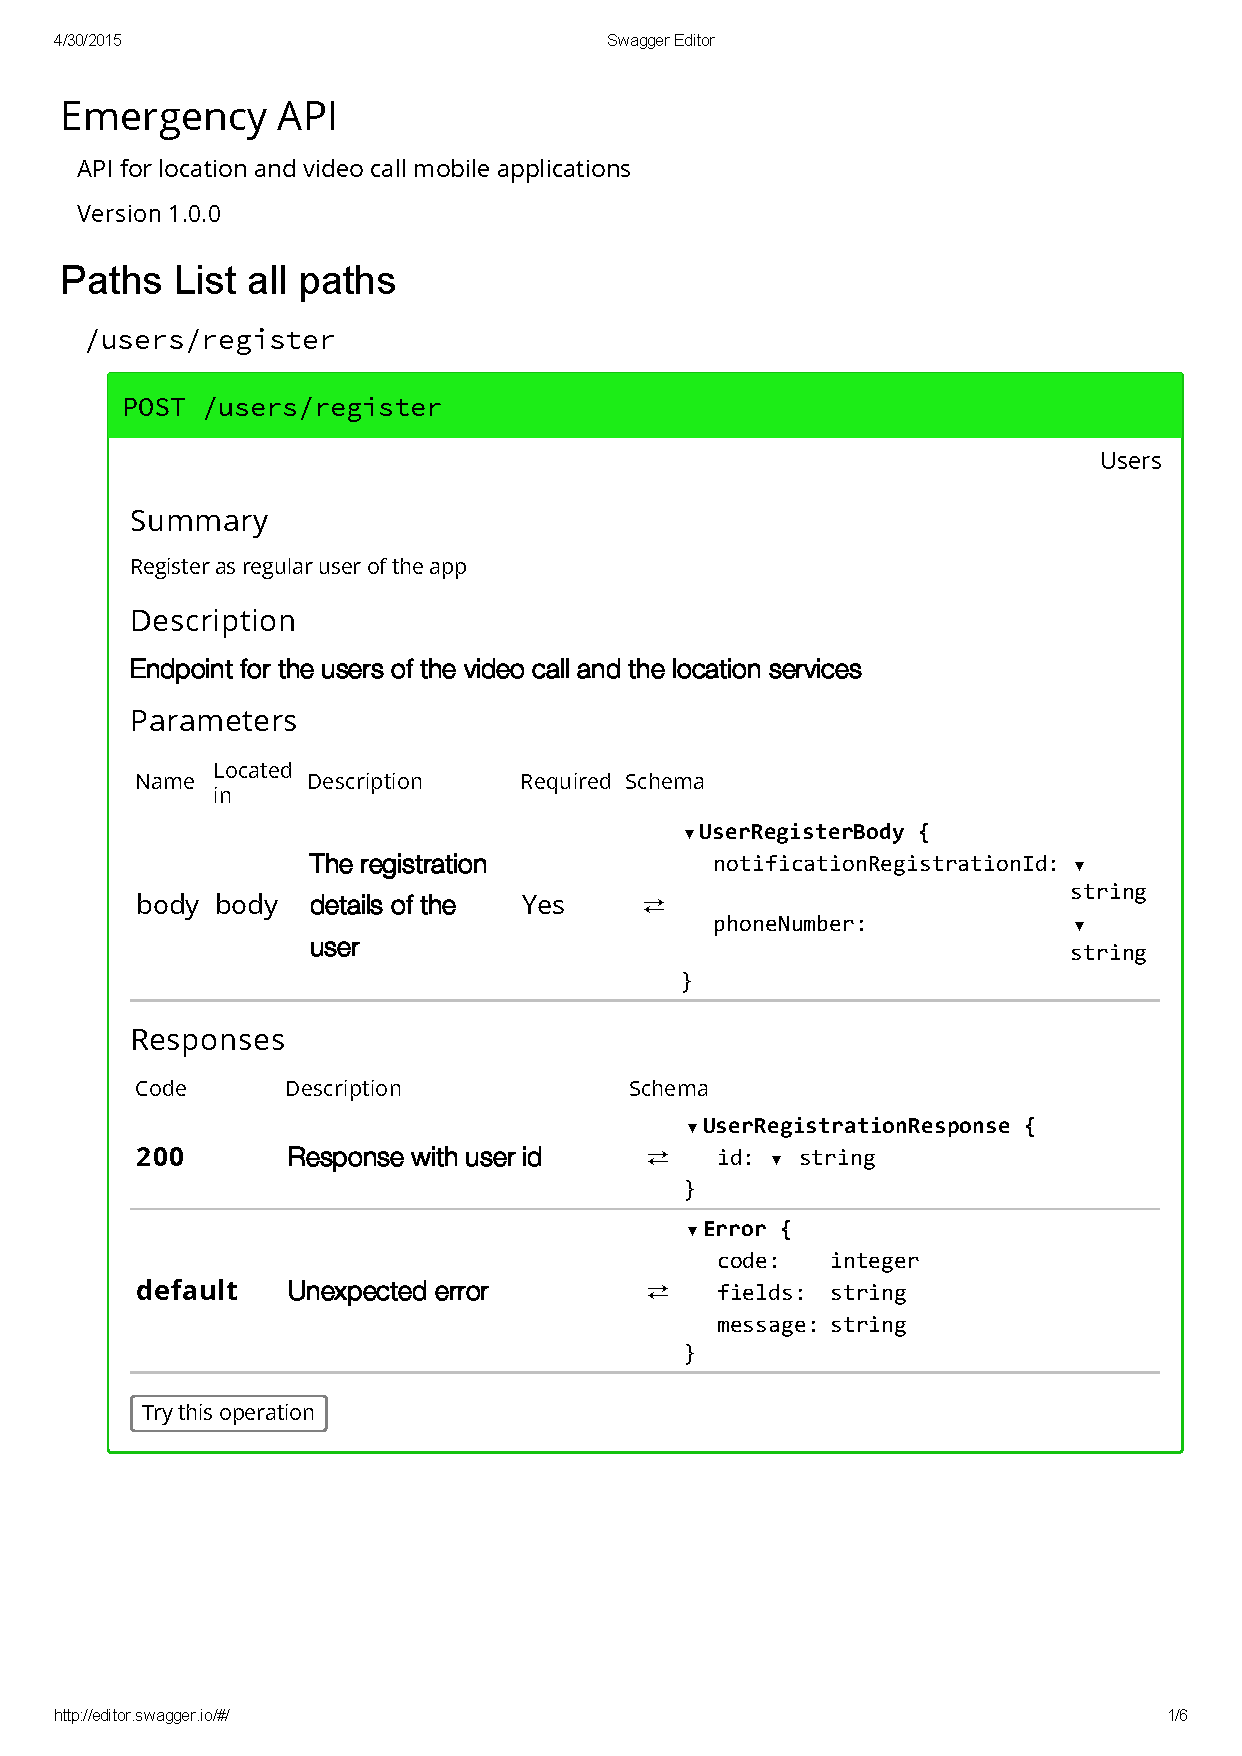
\includepdf[pages={-}]{API/EmergencyClient.pdf}
\begin{figure}[htp] \centering{
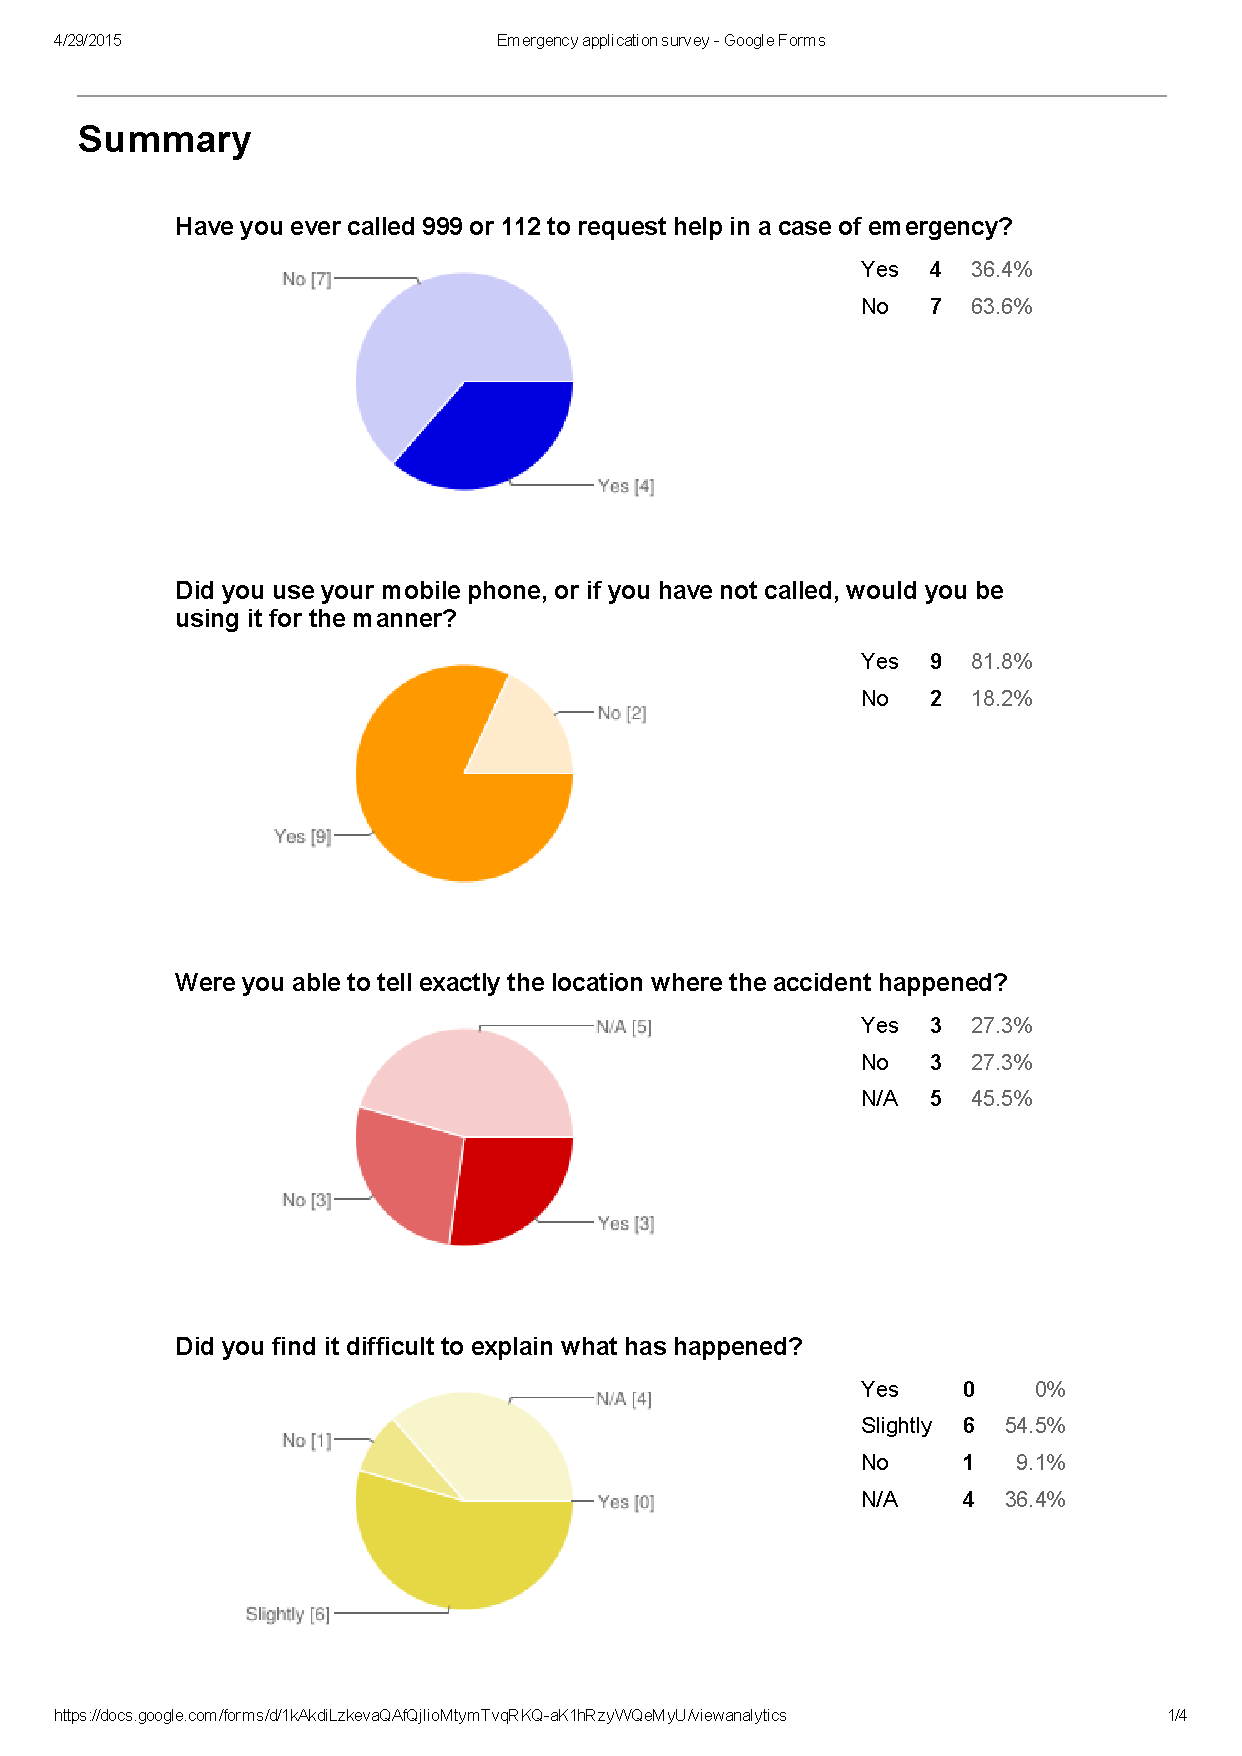
\includepdf[pages={1},scale=0.9,offset=0 -15mm,clip,trim=0mm 25.2mm 0mm 30mm]{Survey/Emergencyapplicationsurvey-GoogleForms.pdf}}
\end{figure}
\pagebreak

    \includepdf[pages={2-},clip,trim=0mm 10mm 0mm 10mm]{Survey/Emergencyapplicationsurvey-GoogleForms.pdf} 
	
	\subsection{Emergency App Database}
	
	\begin{figure}[H]
		\centering
		\includegraphics[width=.9\textwidth]{"VideoStream/database"}
		
		Database for the Emergency App
	\end{figure} \clearpage
	
    \subsection{Video Stream}
    \paragraph{Iteration 1} Appendices for iteration 1.
    
	\begin{figure}[H]
		\centering
		\includegraphics[width=.9\textwidth]{"VideoStream/1"}

		Sequence diagram for creating an Incident by the operator:
	\end{figure} \clearpage
	
	
	\begin{figure}[h]
		\centering
		\includegraphics[width=.9\textwidth]{"VideoStream/2"}

		Sequence diagram for requesting the start of a video stream by the operator:
	\end{figure} \clearpage
	
	
	\begin{figure}[h]
		\centering
		\includegraphics[width=.9\textwidth]{"VideoStream/3"}

		
	\end{figure} \clearpage
	
	
	
	\begin{figure}
\centering
\begin{subfigure}{.5\textwidth}
  \centering
  \includegraphics[width=.9\linewidth]{"VideoStream/4"}
  
  Sequence diagram for starting the video stream by the user:
\end{subfigure}%
\begin{subfigure}{.5\textwidth}
  \centering
  \includegraphics[width=.9\linewidth]{"VideoStream/5"}
	
	Mobile application screen showing the confirm dialog for starting the video stream:
\end{subfigure}
\end{figure}
	\clearpage
	
	
	
	\begin{figure}
\centering
\begin{subfigure}{.5\textwidth}
  \centering
  \includegraphics[width=.9\linewidth]{"VideoStream/6"}
  
  Sequence diagram for starting the video stream by the user:
\end{subfigure}%
\begin{subfigure}{.5\textwidth}
  \centering
  \includegraphics[width=.9\linewidth]{"VideoStream/7"}
	
	Mobile application screen showing the confirm dialog for starting the video stream:
\end{subfigure}
\end{figure}
	
	
	\begin{figure}[h]
		\centering
		\includegraphics[width=.9\textwidth]{"VideoStream/8"}

UI for the operator, providing functionality of searching for a phone number, in order to start an Incident session.
	\end{figure} 
	
	\begin{figure}[h]
		\centering
		\includegraphics[width=.9\textwidth]{"VideoStream/9"}

UI for the operator to request the start of a video stream, once a session has been initiated.
	\end{figure}\clearpage
	
	\begin{figure}[h]
		\centering
		\includegraphics[width=.9\textwidth]{"VideoStream/10"}

UI for the operator, in order to see the live stream and to stop the stream:
	\end{figure}\clearpage
%-------------------------------------------------------------------
    
    \subsubsection{Iteration 2} Appendices for iteration 2.
	
	\begin{figure}[h]
		\centering
		\includegraphics[width=.9\textwidth]{"VideoStream/11"}

		UI during video stream for devices with front-camera and flashlight.
	\end{figure} \clearpage
    
    
	
	\begin{figure}[h]
		\centering
		\includegraphics[width=.9\textwidth]{"VideoStream/12"}

		UI during video stream for devices without front-camera but with flashlight.
	\end{figure} \clearpage
    
    
	
	\begin{figure}[h]
		\centering
		\includegraphics[width=.9\textwidth]{"VideoStream/13"}

		UI during video stream for devices with front-camera but without flashlight.
	\end{figure} \clearpage
    
    
	
	\begin{figure}[h]
		\centering
		\includegraphics[width=.9\textwidth]{"VideoStream/14"}

		UI during video stream for devices without front-camera and flashlight.
	\end{figure} \clearpage
    
    
	
	\begin{figure}[h]
		\centering
		\includegraphics[width=.6\textwidth]{"VideoStream/15"}

		UI for setting the prefered video streaming quality during a video stream. Also available from main menu screen.
	\end{figure} \clearpage
    
    
	
	\begin{figure}[h]
		\centering
		\includegraphics[width=.6\textwidth]{"VideoStream/16"}

		Main Menu screen of the mobile app:
	\end{figure} \clearpage
    
%----------------------------------------------------------------
%iteration 3
	
    \subsubsection{Iteration 3} Appendices for iteration 3.
	\begin{figure}[h]
		\centering
		\includegraphics[width=.9\textwidth]{"VideoStream/17"}

		Backend for searching old incidents:
		
	\vspace{-5pt}
	\end{figure}
    
    
	
	\begin{figure}[h]
		\centering
	\vspace{-10pt}
		\includegraphics[width=.8\textwidth]{"VideoStream/18"}

		UI for the operator to skip/seek video:
	\vspace{-60pt}
	\end{figure} \clearpage
	    %---------------------------------------------------------------

    \subsubsection{Iteration 4} Appendices for iteration 4.    
	
	\begin{figure}[h]
		\centering
		\includegraphics[width=.8\textwidth]{"VideoStream/19"}

		Confirmation dialog on back press, asking for closing the incident session, leaving it open or going back to the screen:
	\vspace{-5pt}
	\end{figure}
    
    
	
	\begin{figure}[h]
		\centering
	\vspace{-10pt}
		\includegraphics[width=.8\textwidth]{"VideoStream/20"}

		UI screen to show a currently opened session:
	\vspace{-60pt}
	\end{figure} \clearpage
	
	
	e%---------------------------------------------------------------

\subsubsection{Iteration 4} Appendices for iteration 4.    
	
    	
	\begin{figure}[h]
		\centering
		\includegraphics[width=.8\textwidth]{"VideoStream/21"}

		UI to show that more video streams are available for the current incident:
	\vspace{-5pt}
	\end{figure}
    
    
	
	\begin{figure}[h]
		\centering
	\vspace{-5pt}
		\includegraphics[width=.8\textwidth]{"VideoStream/22"}

		UI to show current available streams for the current incident.
	\vspace{-60pt}
	\end{figure}
	\pagebreak
	\clearpage
	
	





	
    \subsection{Chat}
    \subsubsection{Iteration 1} Appendices for iteration 1.
    
	\begin{figure}[h]
		\centering
		\includegraphics[width=.5\textwidth]{"Chat/1"}

  Mobile application Main Menu for starting a chat:
	\end{figure} \clearpage
	
	
	\begin{figure}[h]
		\centering
		\includegraphics[width=.6\textwidth]{"Chat/2"}

	Mobile application UI for the live chat:
	\end{figure} \clearpage
	
	
	\begin{figure}[h]
	\vspace{-30pt}
		\centering
		\includegraphics[width=.8\textwidth]{"Chat/3"}

		Backend UI for showing currently pending chats:
	\end{figure} 
	
	
	\begin{figure}[h]
		\centering
		\includegraphics[width=.8\textwidth]{"Chat/4"}

		UI for showing chat in an active incident session:
	\vspace{-30pt}
	\end{figure} \clearpage
	
	
	\begin{figure}[h]
	\vspace{-30pt}
		\centering
		\includegraphics[width=.8\textwidth]{"Chat/5"}

		UI for Chat with multiple video streams available:
	\end{figure} 
	
	\begin{figure}[h]
		\centering
		\includegraphics[width=.8\textwidth]{"Chat/6"}

		UI for Chat with multiple video streams available:

	\vspace{-30pt}
	\end{figure} \clearpage
	
    \subsubsection{Iteration 2} Appendices for iteration 2.

	
	\begin{figure}[h]
\centering
\begin{subfigure}{.5\textwidth}
  \centering
  \includegraphics[width=.9\linewidth]{"Chat/7"}
  
		Confirmation dialog for starting a live chat:
\end{subfigure}%
\begin{subfigure}{.5\textwidth}
  \centering
  \includegraphics[width=.9\linewidth]{"Chat/8"}
	
	Video stream UI for switching to chat and new messages indicator:
\end{subfigure}
\end{figure}	
\clearpage



	\begin{figure}
\centering
\begin{subfigure}{.5\textwidth}
  \centering
  \includegraphics[width=.9\linewidth]{"Chat/9"}
  
		The chat screen with a button for starting a video stream and sending the location:
\end{subfigure}%
\begin{subfigure}{.5\textwidth}
  \centering
  \includegraphics[width=.9\linewidth]{"Chat/10"}
	
	Video stream UI for switching to chat and new messages indicator:
\end{subfigure}
\end{figure}\clearpage










	
    \subsection{Automatic Video Sending}
    \subsubsection{Iteration 1} Appendices for iteration 1.
    


	\begin{figure}[h]
		\centering
		\includegraphics[width=1\textwidth]{"Auto/1"}

		Deployment Diagram:
	\end{figure}
	
	
	
	
	\begin{figure}[h]
		\centering
		\includegraphics[width=1\textwidth]{"Auto/2"}

		Class diagram:
	\end{figure} \clearpage
	
	
	
	
	
	\begin{figure}[h]
		\centering
		\includegraphics[width=.6\textwidth]{"Auto/3"}

		Mobile application confirm dialog for sending the current location:
	\end{figure} \clearpage
	
	
	\begin{figure}[h]
	\vspace{-30pt}
		\centering
		\includegraphics[width=.8\textwidth]{"Auto/4"}

		Request location button in the backend UI:

	\end{figure}
	
	
	\begin{figure}[h]
		\centering
		\includegraphics[width=.8\textwidth]{"Auto/5"}

		Location received on backend UI:
	\vspace{-30pt}
	\end{figure} \clearpage
	
		
	
	
    \subsection{API for Client \& Server}
    %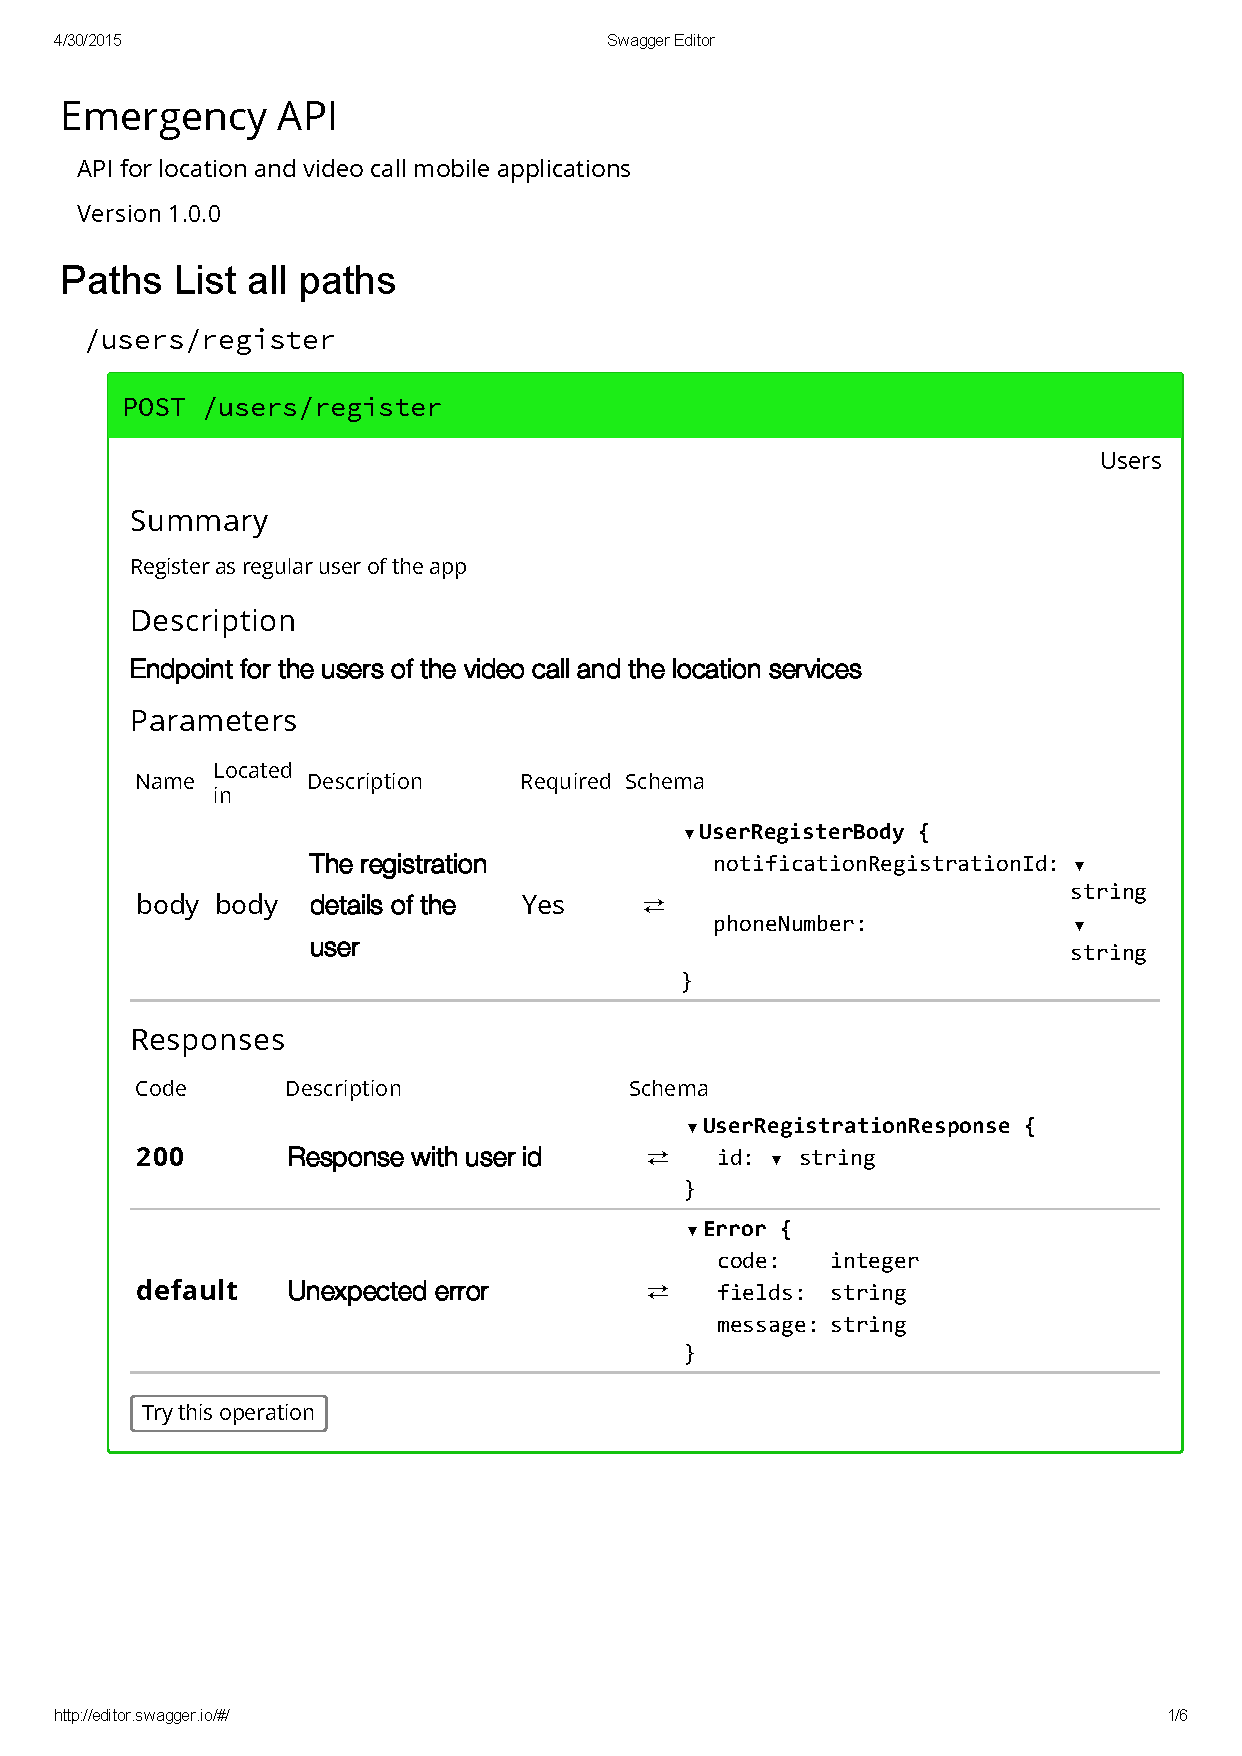
\includepdf[pages={-}]{API/EmergencyClient.pdf}
\begin{figure}[htp] \centering{
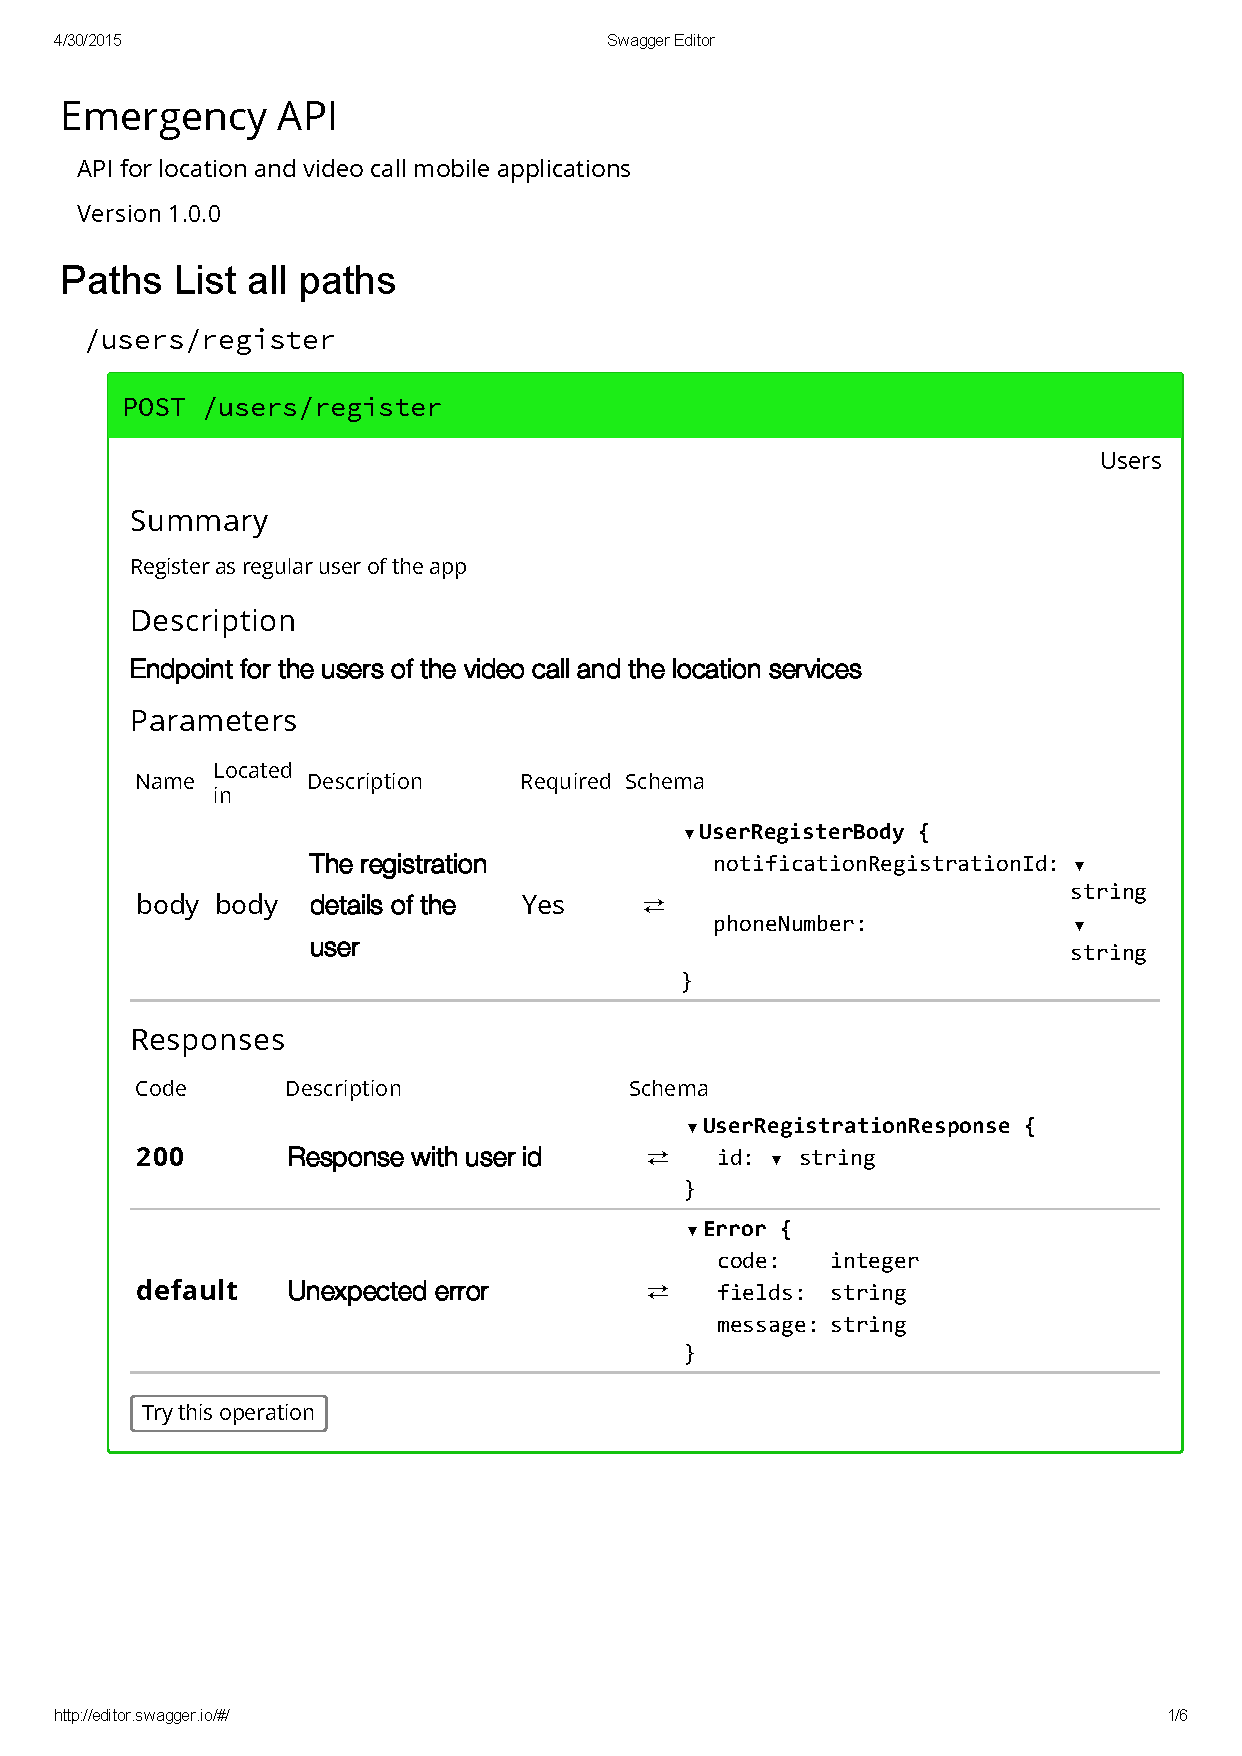
\includepdf[pages={1},offset={0 -130}]{API/EmergencyClient.pdf}}
\end{figure}
\pagebreak

    \includepdf[pages={2-},pagecommand=\thispagestyle{plain},clip,trim=0mm 10mm 0mm 10mm]{API/EmergencyClient.pdf}
    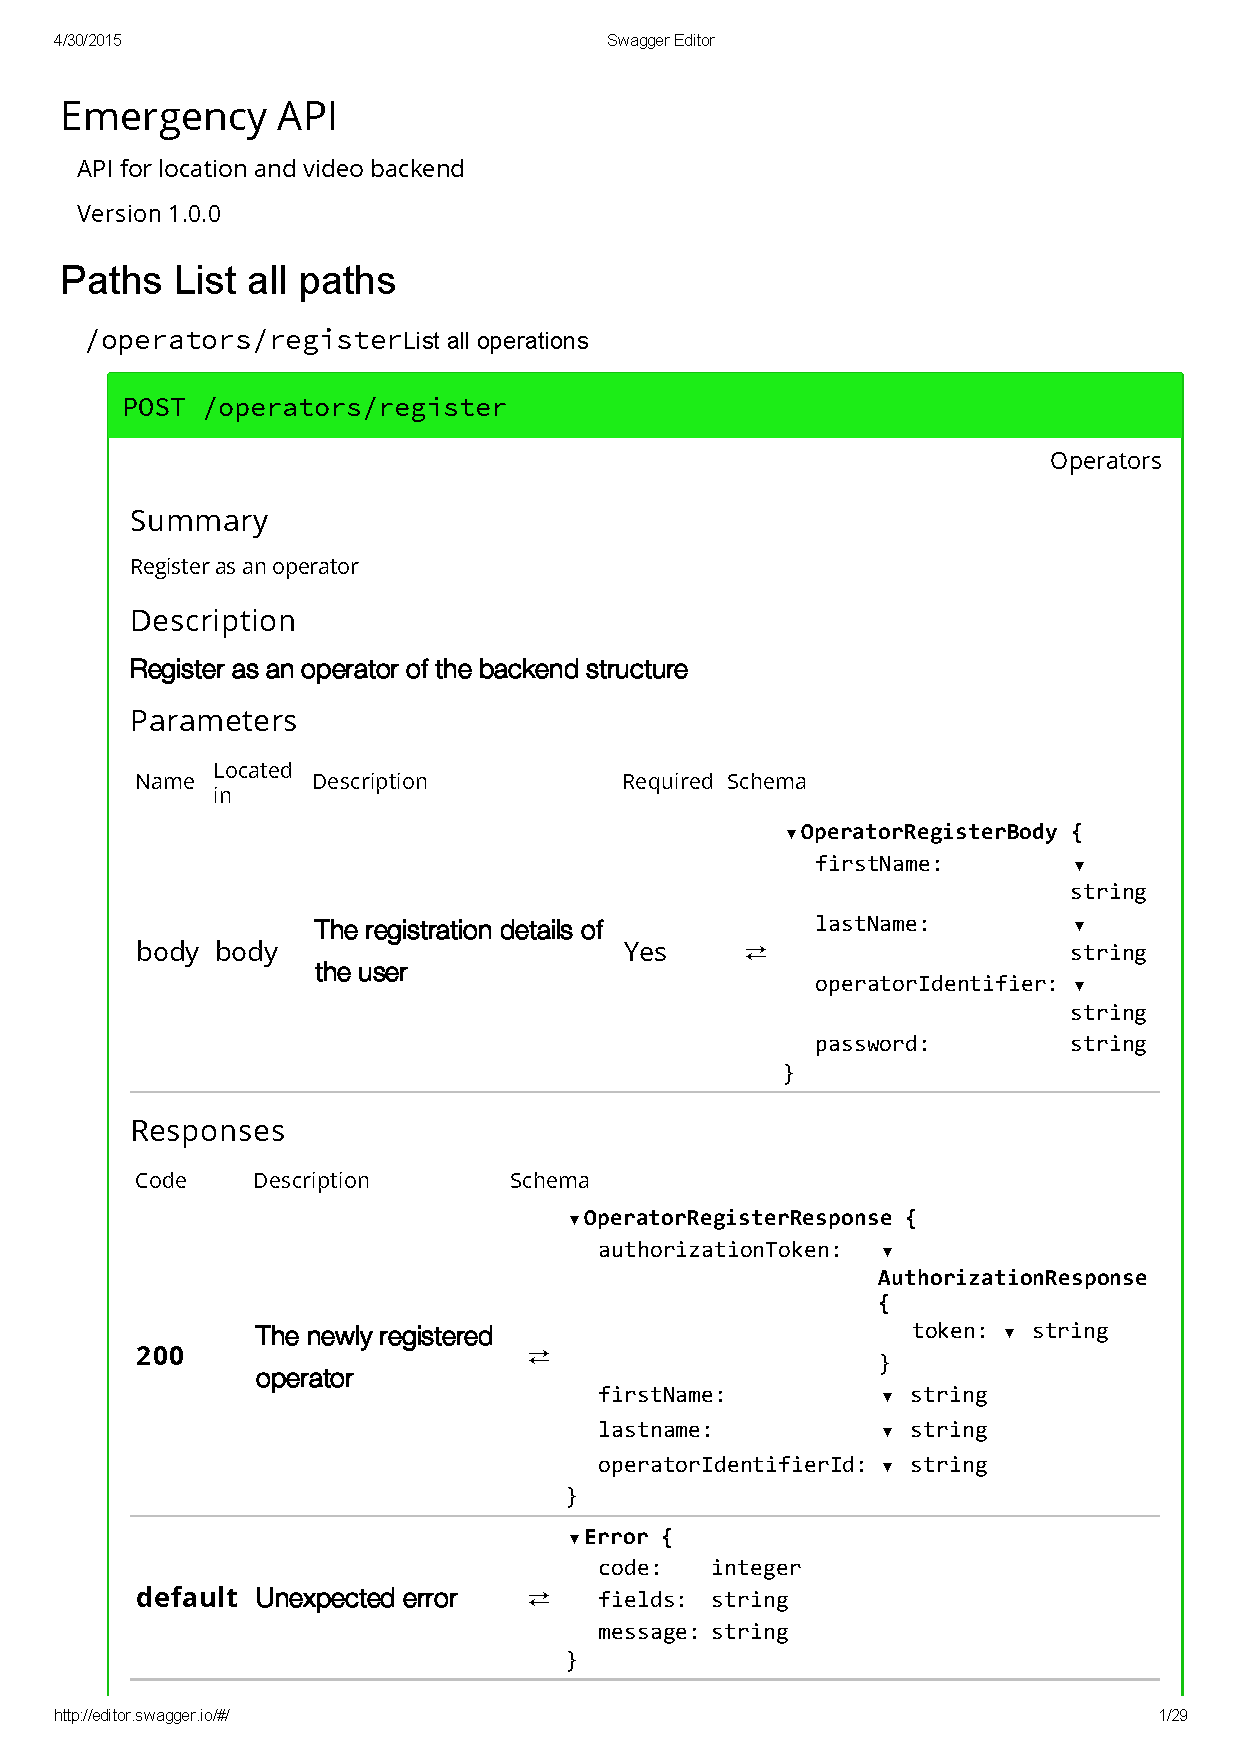
\includepdf[pages={-},pagecommand=\thispagestyle{plain},clip,trim=0mm 10mm 0mm 10mm]{API/EmergencyServer.pdf}


	
	
\end{document}